\documentclass[10pt]{beamer}
\usepackage{algpseudocode}
\usepackage[linesnumbered,ruled,vlined]{algorithm2e}
\usepackage{graphicx}
\usepackage{wrapfig}
\usepackage{xeCJK}
\setCJKmainfont{Songti SC}[%
UprightFont    = * Light,
BoldFont       = * Bold,
ItalicFont     = Kaiti SC,
BoldItalicFont = Kaiti SC Bold,
]
\setCJKsansfont{STFangsong}[BoldFont = * Medium]%
\setCJKmonofont{STFangsong}%
\mode<beamer>{%
  \usetheme[hideothersubsections,
            left,width=22mm]{Berkeley}
  % \usecolortheme[]{}
}
\usepackage[most]{tcolorbox}

\usepackage{caption}
\captionsetup[figure]{labelformat=empty}% redefines the caption setup of the figures environment in the beamer class.

\setbeamertemplate{footline}[frame number]

\usepackage{varwidth}    
\usepackage{etoolbox}
\makeatletter
%\patchcmd{\beamer@sectionintoc}{\vskip1.5em}{\vskip0.5em}{}{}
\patchcmd{\beamer@sectionintoc}{%
  \hbox{\vbox{%
    \def\beamer@breakhere{\\}%
    \beamer@tocact{\ifnum\c@section=#1\beamer@toc@cs\else\beamer@toc@os\fi}{section in toc}}}%
}{%
  \hbox{%
    \def\beamer@breakhere{}%
    \beamer@tocact{\ifnum\c@section=#1\beamer@toc@cs\else\beamer@toc@os\fi}{section in toc}}%
}{}{}
\makeatother    
\setbeamertemplate{section in toc}[sections numbered]    


\title{面向分布式图计算系统的自适应优化方法研究}
\author[Junhang Chen]{陈军航}
% \institute[ucas]{中国科学院大学}
\titlegraphic{
\includegraphics[width=30mm]{UCAS.png}}

\date{\today}
\begin{document}
  
\begin{frame}%title
  \titlepage
\end{frame}

\begin{frame}%toc
  \begin{center}
  \begin{varwidth}{\textwidth}
  \tableofcontents[sectionstyle=show,subsectionstyle=show] 
  \end{varwidth}
  \end{center}
\end{frame}

\section{研究背景-分布式图计算中的延迟数据一致性方法(LazyAsync)}


\begin{frame}% 引入图计算的定义,和它的重要性
  \frametitle{研究背景-图计算}
    \begin{block}
      {图结构的数据与分布式图计算}
      \begin{itemize}
        \item 很多问题都能抽象出图模型,很多领域都产生图数据
        \begin{figure}[!htbp]
          \centering
          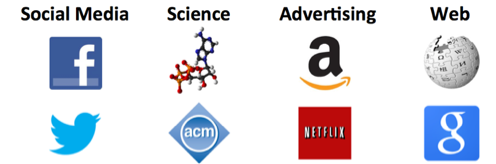
\includegraphics[width=0.60\textwidth]{Img/graphs_are_everywhere.png}
          % \caption{图计算的应用领域}
          \label{fig:graph_important}
        \end{figure}
      \end{itemize}
      \begin{itemize}
        \item 随着数据规模的不断扩大,人们开发了各种分布式图计算系统
        \begin{itemize}
          \item Pregel,Google
          \item PowerGraph,CMU
          \item Gemini,Tsinghua
          \item GraphX,Apache
          \item \ldots 
        \end{itemize}
      \end{itemize}
    \end{block}
\end{frame}


\begin{frame}%什么是副本点
  \frametitle{分布式图计算系统中的副本点}
  \begin{block}
    {副本点及它的数据一致性问题(data coherency)}
    \begin{figure}[!htbp]
      \centering
      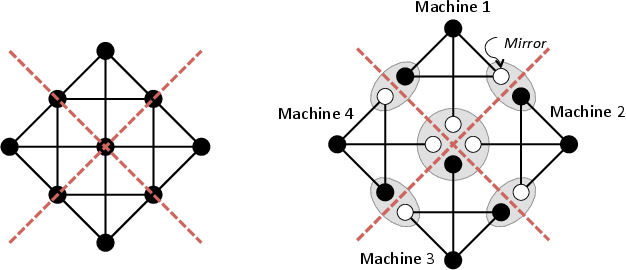
\includegraphics[width=0.8\textwidth]{Img/mirror}
      \label{fig:mirror}
    \end{figure}
  \end{block}
\end{frame}


\begin{frame}%急切与延迟数据一致性
  \frametitle{分布式图计算系统如何处理副本点之间的数据一致性问题}
  \begin{block}
    {急切数据一致性(eager data coherency)方法}
    \begin{figure}[!htbp]
      \centering
      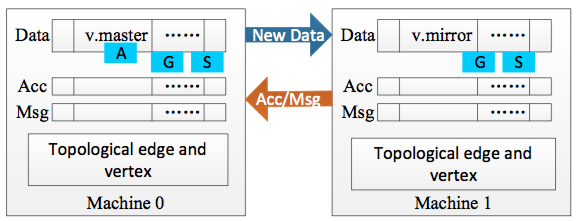
\includegraphics[width=0.40\textwidth]{Img/pg-eager}
    \end{figure}
  \end{block}
  \begin{block}
    {延迟数据一致性(lazy data coherency)方法}
    \begin{figure}[!htbp]
      \centering
      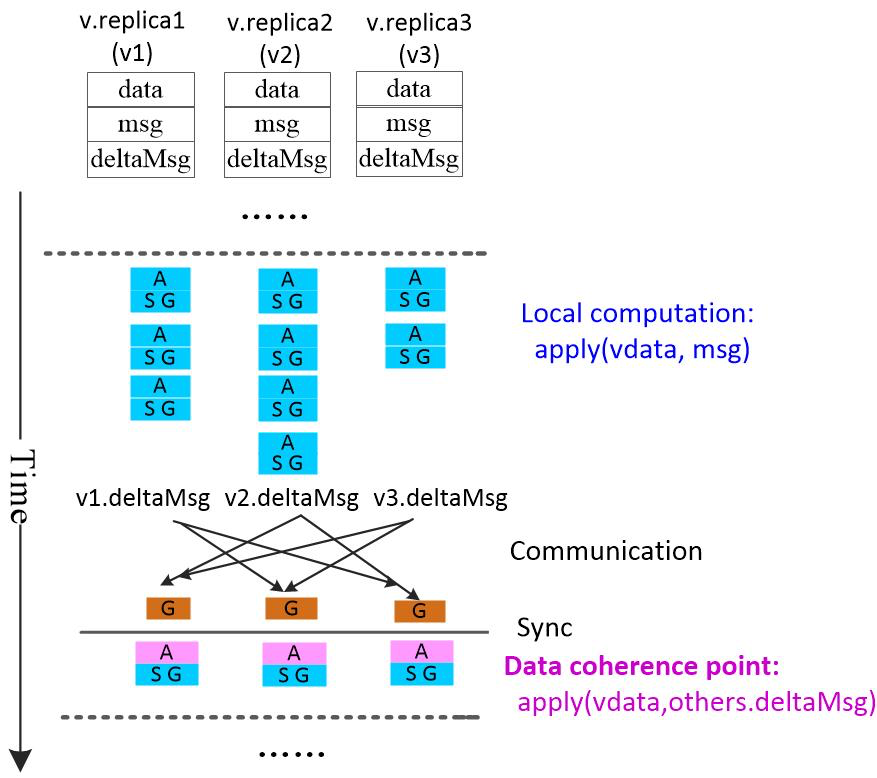
\includegraphics[height=0.3\textwidth]{Img/lazy_data_coherency.png}
    \end{figure}
  \end{block}
\end{frame}


\begin{frame}%介绍我们的延迟一致性  
  \frametitle{延迟数据一致性方法(LazyAsync)的效果}
  \vspace{-1em}
  延迟数据一致性方法,在保留副本点带来的好处的同时,降低系统由于维护副本点间数据一致性带来的开销。
  实验结果表明这种方法极大地提升了分布式图计算系统的处理能力。相关成果最终发表在PPoPP'18 CCF A类会议上。
  \vspace{-1em}
  \begin{figure}
    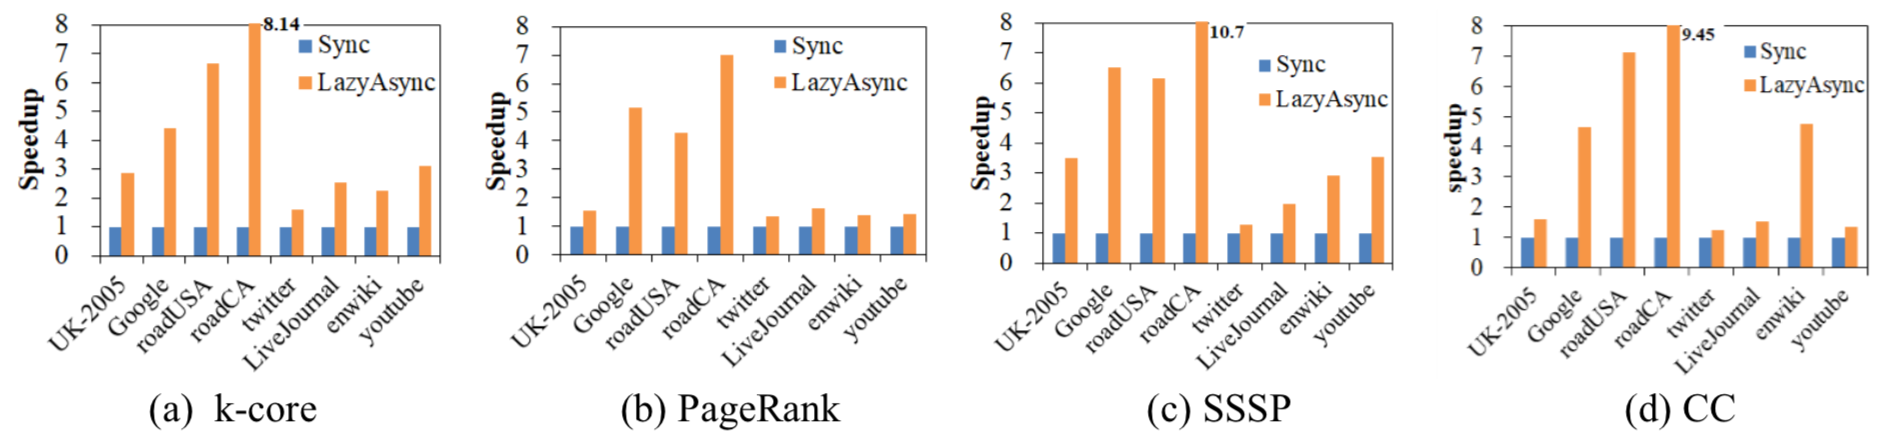
\includegraphics[scale=0.3]{Img/speedup.png}
    \caption{48机下4种算法在不同真实图上的加速比对比}  
  \end{figure}

  % % \vspace{-2em}
  % \begin{tcolorbox}[boxrule=0.2mm,breakable,arc = 0mm, colback = white,colframe=black]
  % Lei Wang, Liangji Zhuang, \underline{Junhang Chen}, et al. \\
  % LazyGraph: Lazy Data Coherency for Replicas in Distributed Graph-Parallel Computation. In PPoPP, 2018.  
  % \end{tcolorbox}
\end{frame}

\section{研究动机-LazyAsync 如何自适应调优}


\begin{frame}%lazyasync 问题1:性能波动
  \frametitle{LazyAsync 的开启策略问题}
  \vspace{-1em}
  \begin{block}
    {开启策略:何时启用延迟数据一致性方法}
    \begin{figure}[!htbp]
      \centering
      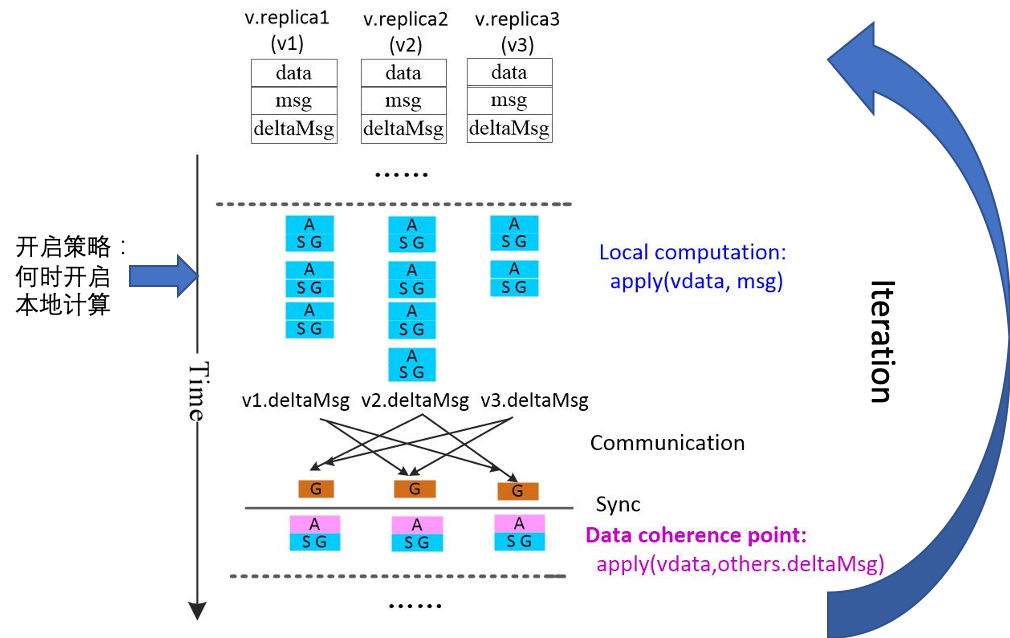
\includegraphics[height=0.5\textwidth]{Img/turn_on.png}
    \end{figure}

    \begin{itemize}
      \item 直接开启还是等待几轮后开启?不同的开启策略会得到不同的性能提升效果,背后的原因是什么?
      \item 怎样选择合适的开启策略从而得到相对最优的性能提升?
    \end{itemize}
  \end{block}
\end{frame}


\begin{frame}%lazyasync 问题2:dt fail 
  \frametitle{存在缺陷的决策树开启策略}
  \begin{columns}
    \begin{column}{0.4\textwidth}
      \centering
      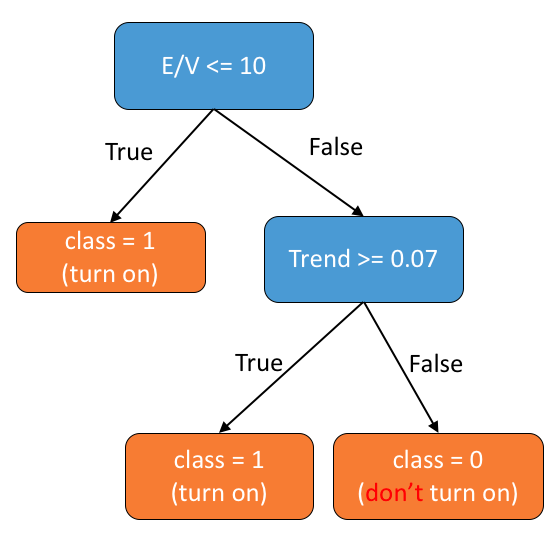
\includegraphics[width=1.0\textwidth]{Img/decision_tree}
    \end{column}
    \begin{column}{0.6\textwidth}  %%<--- here
      \centering
      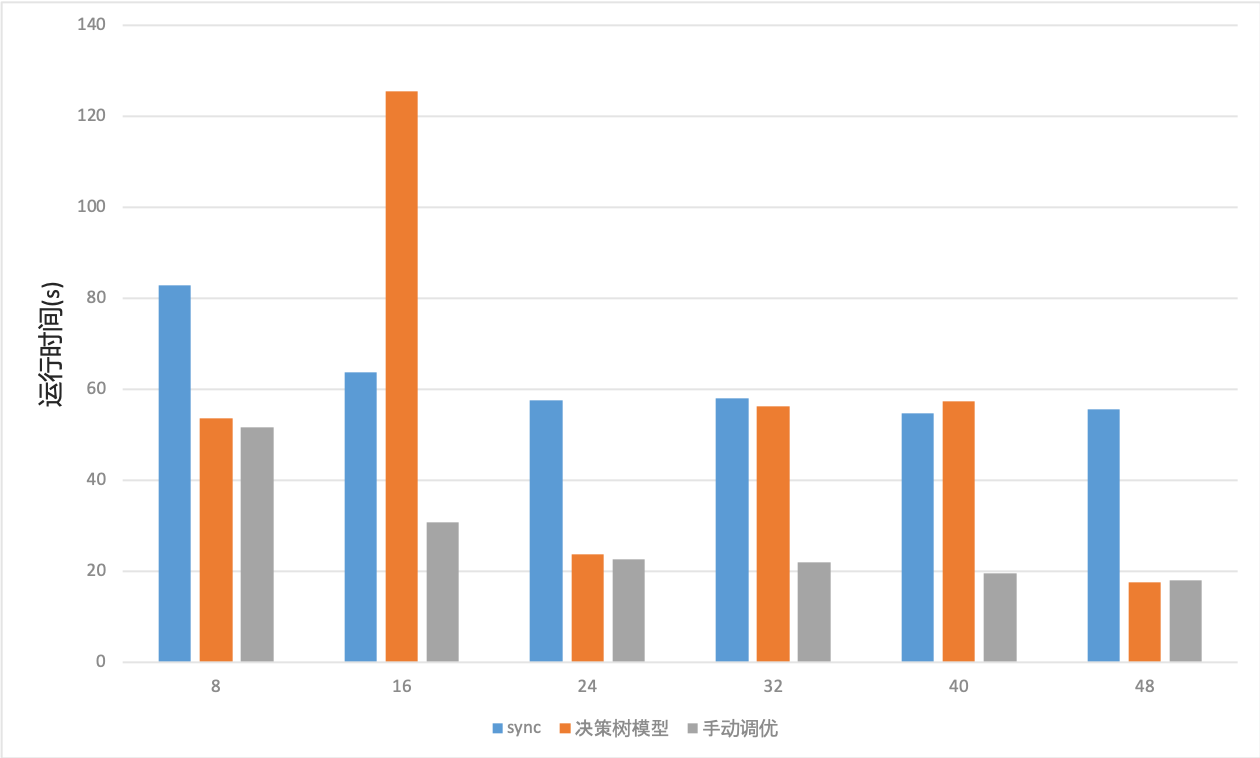
\includegraphics[width=1.0\textwidth]{Img/dtreefail}
    \end{column}
  \end{columns}

  \vspace{2em}

  通过对手动调优产生的组合数据进行拟合训练,我们得到了一个决策树方法。
  这种方法本质上是一种离线方法,并且存在失灵的情况。
\end{frame}

\begin{frame}%lazyasync 需要一个自适应优化方法
  \frametitle{研究动机-LazyAsync 如何自适应调优}
  \begin{block}
    {面向 LazyAsync 的自适应优化方法研究}
    \begin{itemize}
      \item 开启策略如何影响 LazyAsync 的性能提升效果
      \item 如何自动得到相对最优的开启策略\\
      (同时不像决策树方法那样依赖于事先繁重的手动调优工作)
    \end{itemize}
  \end{block}
\end{frame}


\section{研究结果}

\begin{frame}
  \begin{block}
    {面向 LazyAsync 的自适应优化方法研究}
    \begin{itemize}
      \item 开启策略如何影响 LazyAsync 的性能提升效果
      \item 如何自动得到相对最优的开启策略
    \end{itemize}
  \end{block}
  \begin{block}
    {研究结果}
    \begin{enumerate}
      \item 冗余计算是不同开启策略得到不同性能提升这一问题的根源
      \item 图计算过程中存在着解的局部性规律可以减少冗余计算
      \item 基于解的局部性规律实现了一种在线的自适应优化方法\\
      使得 LazyAsync 能够自动得到相对最优的性能提升。
    \end{enumerate}
  \end{block}
\end{frame}
\subsection{1:冗余计算造成LazyAsync性能波动}


\begin{frame}%lazyasync 的性能收益 
  \frametitle{延迟数据一致带来性能收益}
  \begin{figure}[!htbp]
    \centering
    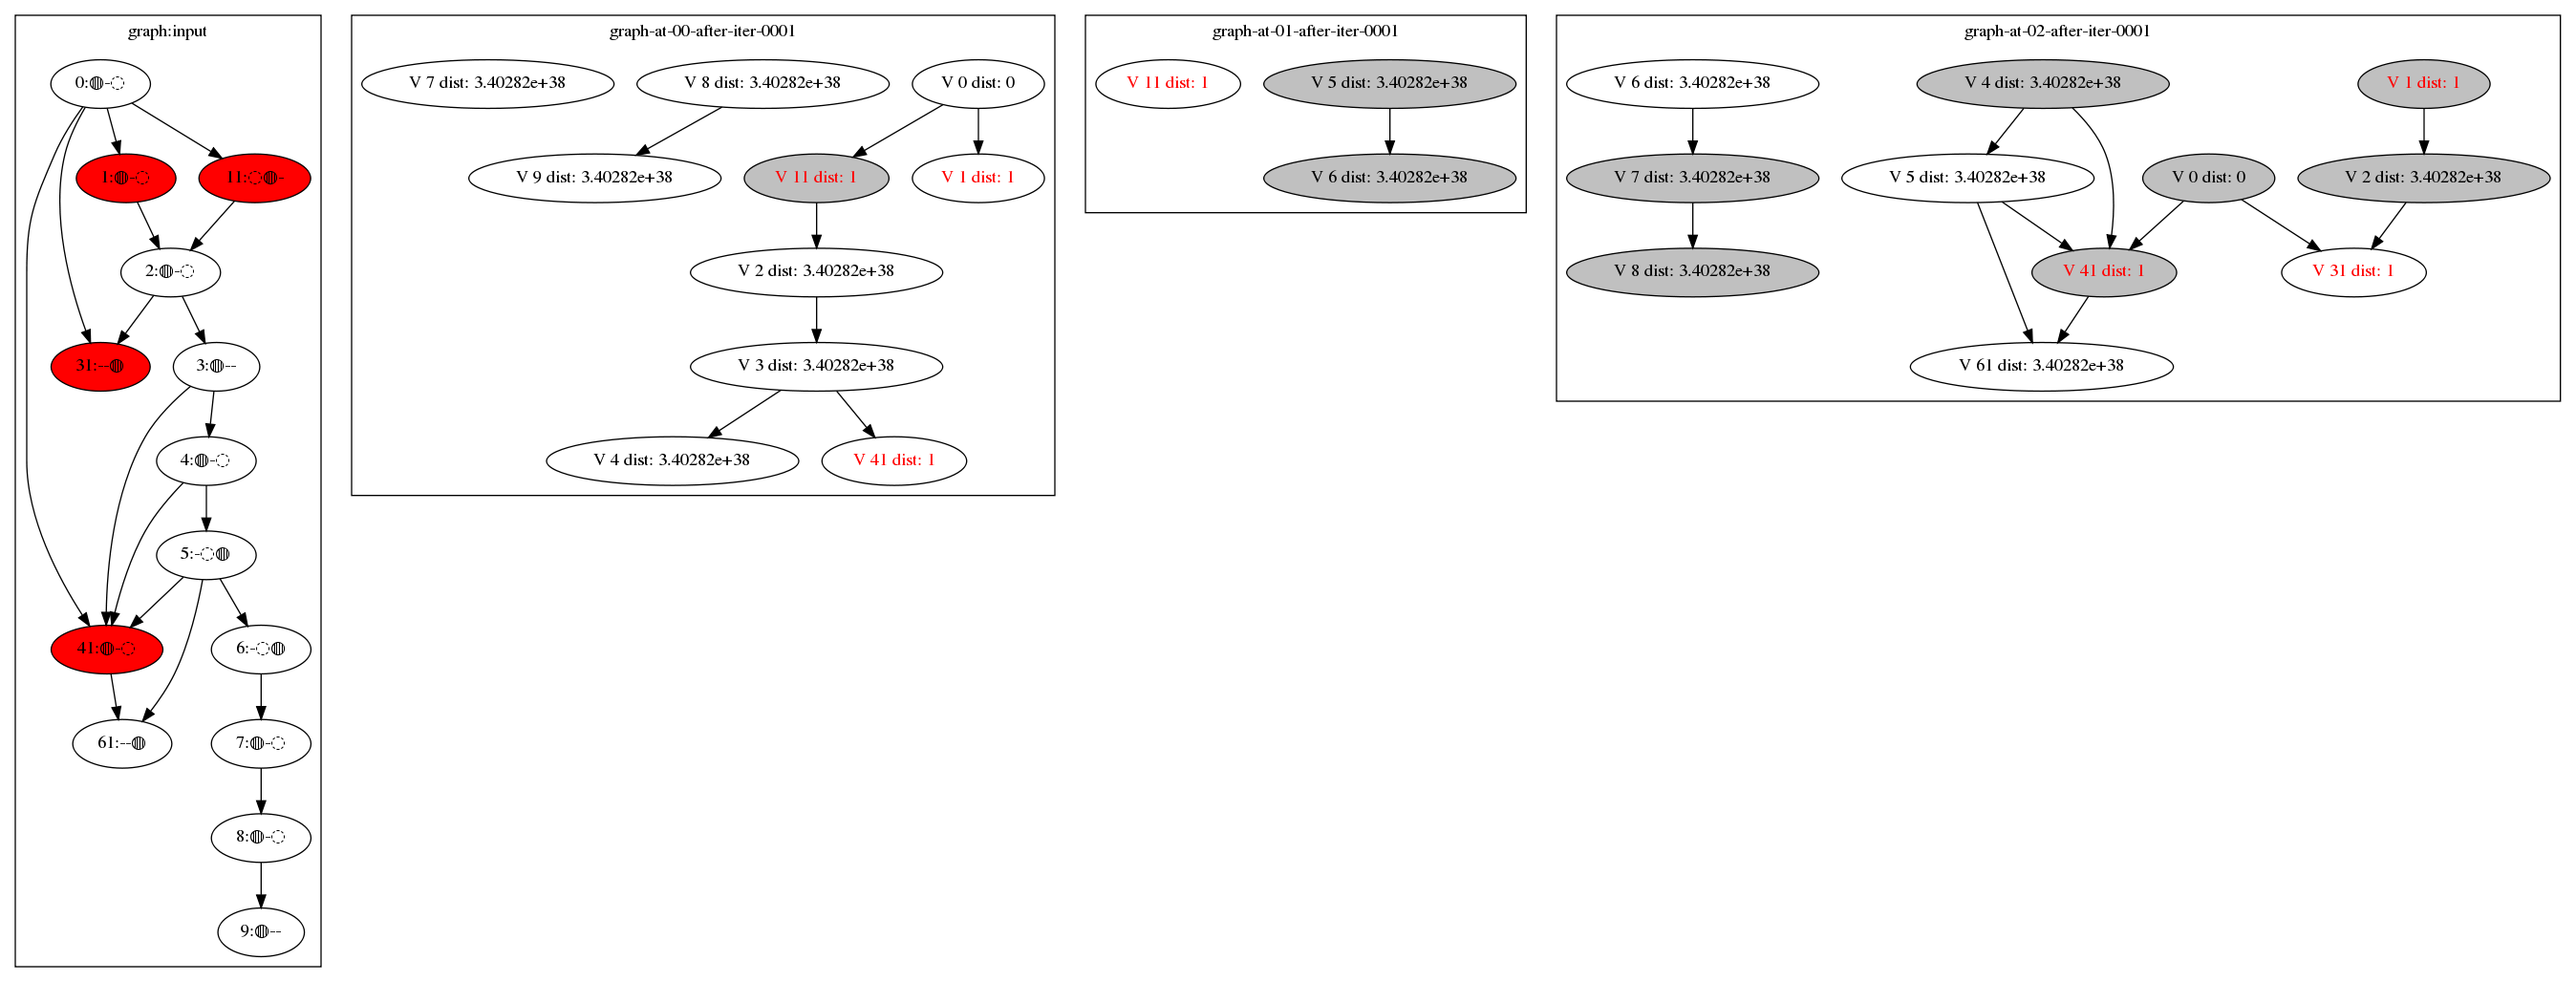
\includegraphics[width=0.8\textwidth]{Img/sync-iter1.png}
    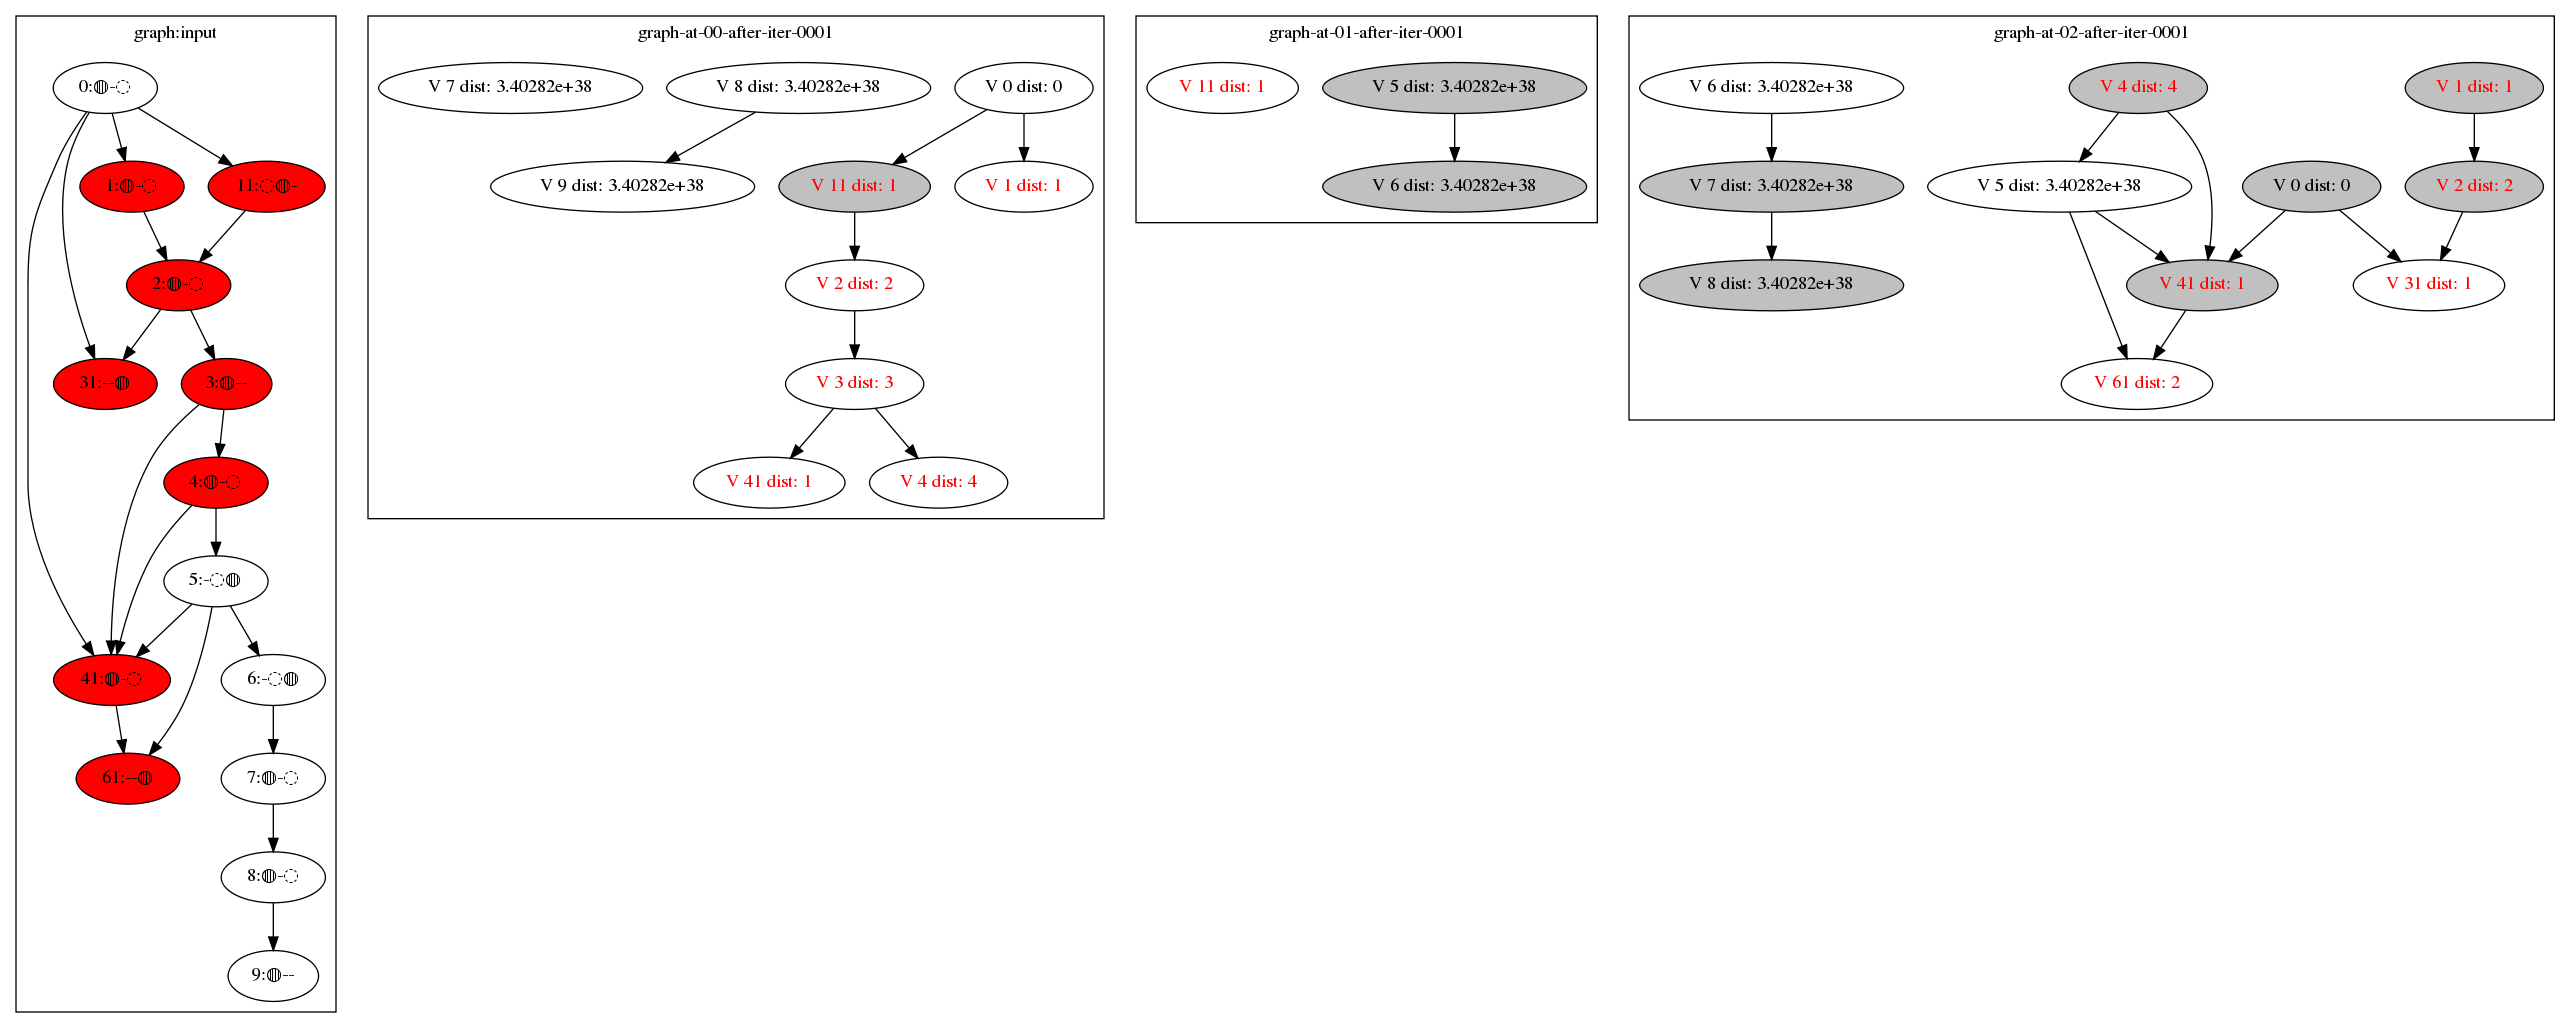
\includegraphics[width=0.8\textwidth]{Img/lazy-iter1.png}
    \caption[]{以 SSSP 为例展示 LazyAsync 的性能收益 }
  \end{figure}
\end{frame}


\begin{frame}%lazyasync 的性能损耗/冗余计算的概念的提出
  \frametitle{冗余计算带来性能损耗} 
  \vspace{-1em}
  \begin{figure}[!htbp]
    \centering
    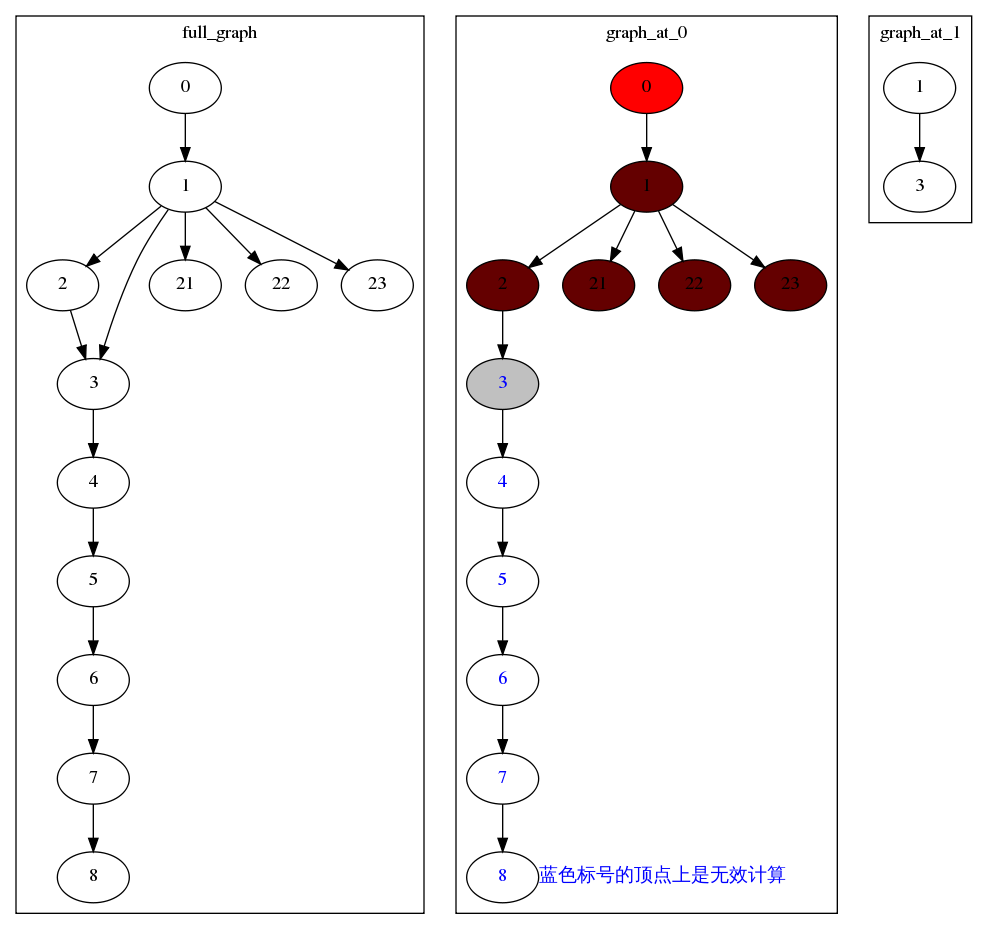
\includegraphics[width=0.7\textwidth]{Img/useless.png}
    \caption[]{有效计算与冗余(无效)计算示意图}
  \end{figure}
\end{frame}

\begin{frame}%如何定性度量冗余计算
  \frametitle{研究冗余计算对LazyAsync的具体影响}
  \begin{block}
    {如何定量地观察冗余计算}
    \begin{itemize}
      \item 先把计算跑完得到最终解
      \item 在顶点上事先记录最终解
      \item 比较迭代解和最终解来判断\\
      一次计算是有效的还是冗余的
    \end{itemize}
  \end{block}

  \vspace{2em}

  解决如何定量度量冗余计算这一问题之后,本文选择 SSSP 算法在4个需要手动调优的输入图上进行了实验,
  来观察不同开启策略下的冗余计算的变化。
\end{frame}

\begin{frame}%实验验证
  \frametitle{实验结果}
  \begin{figure}[!htbp]
    \centering
    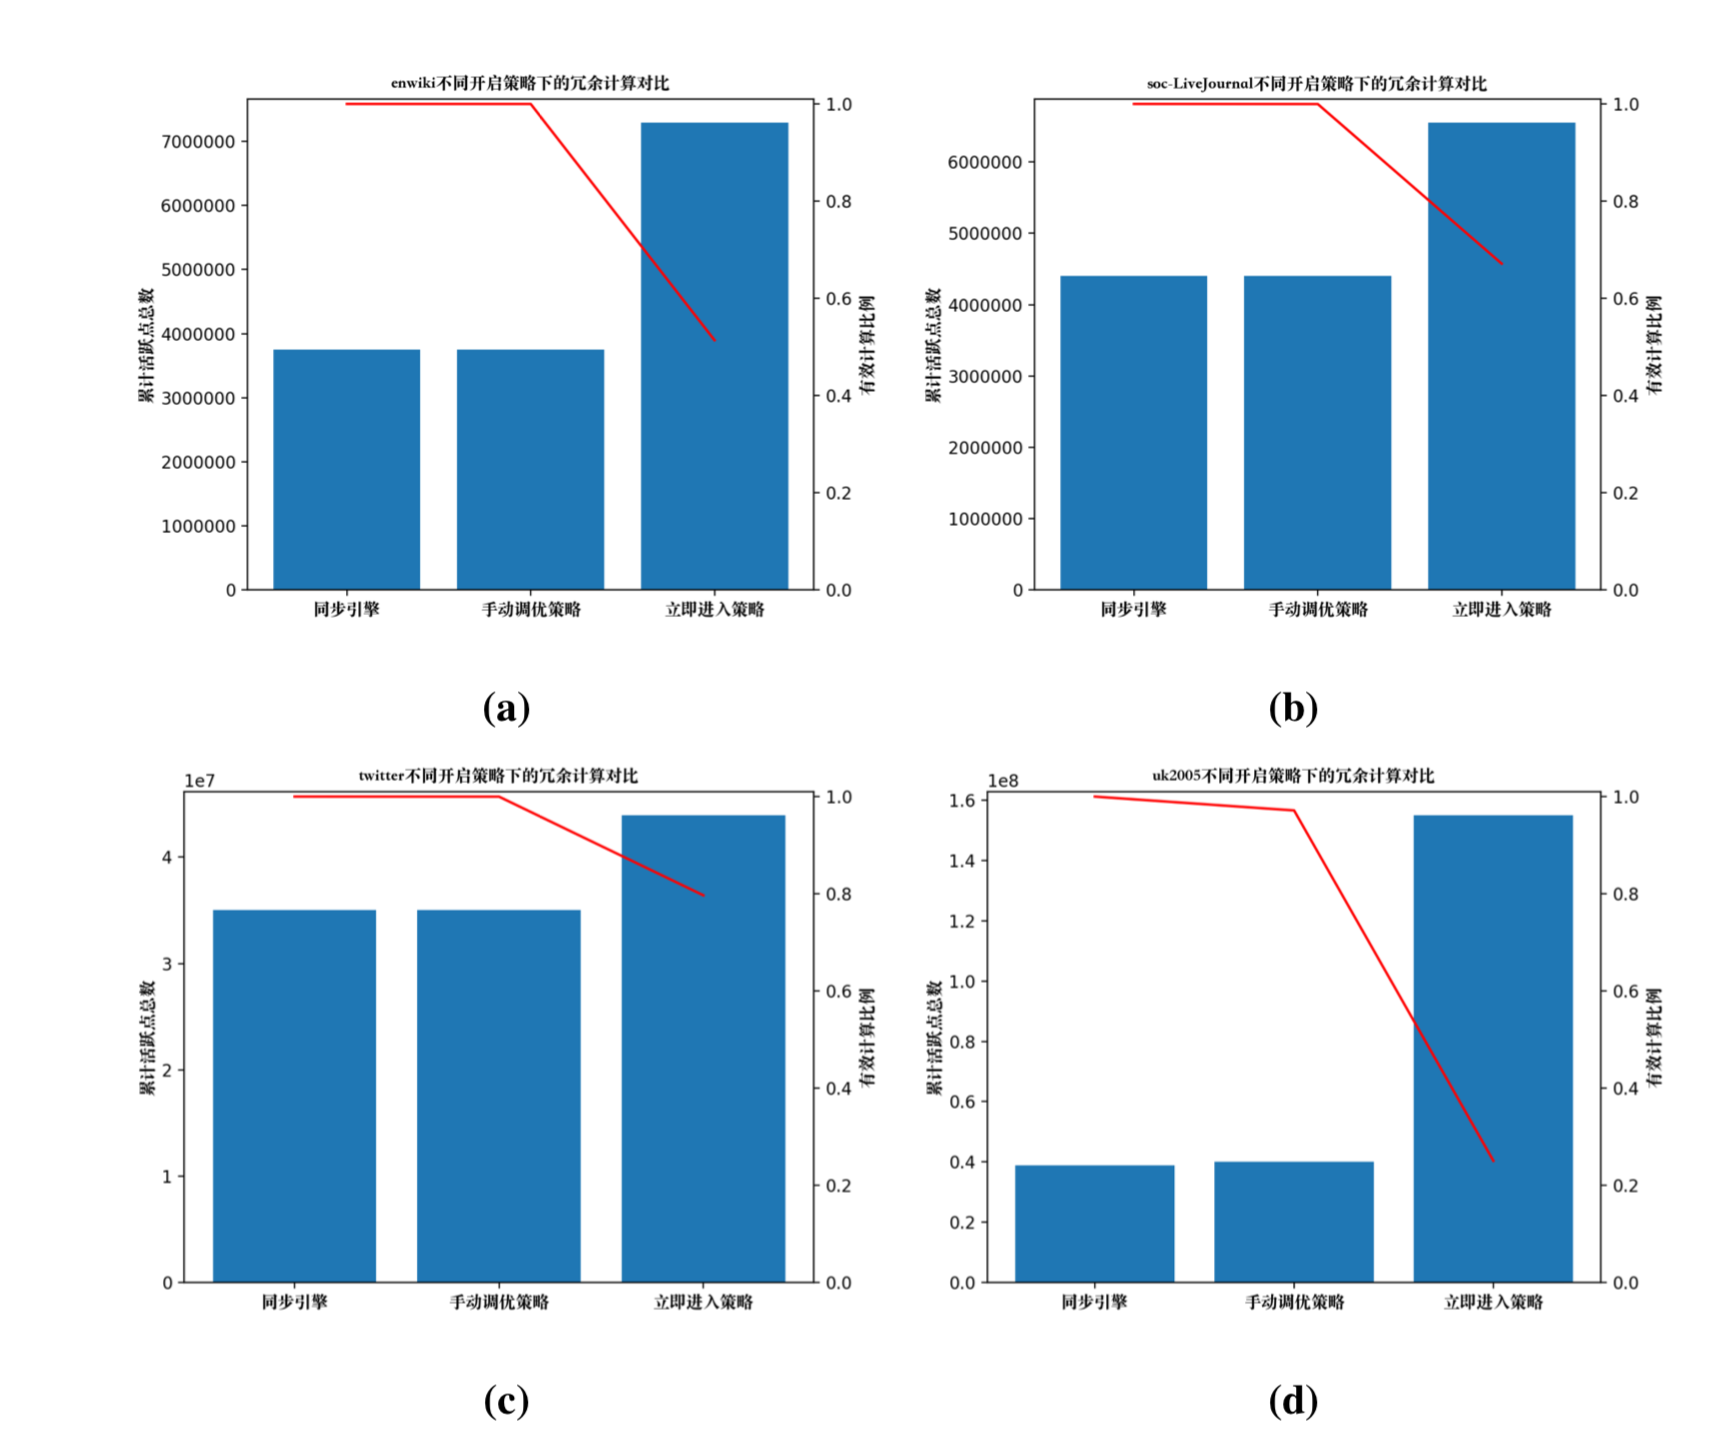
\includegraphics[width=0.8\textwidth]{Img/all_useful.png}
    \caption[]{SSSP在4个输入图上不同开启策略下的冗余计算的比例 }
  \end{figure}
\end{frame}

\begin{frame}%规律总结
  \frametitle{分析与结论}
  \begin{block}
    {实验数据分析}
    \begin{itemize}
      \item 手动调优找到的相对最优的开启策略几乎不存在冗余计算(0.009\%)
      \item 立即进入的开启策略中整体存在着20\%-80\%的冗余计算
      \item 在 enwiki 这个输入图的第2次迭代中,立即进入策略激活并计算了156万个顶点,但只有6万个顶点的计算是有效的,冗余计算的比例达到了96\%
    \end{itemize}
  \end{block}
  大量的冗余计算增加了单次迭代的时间,但带来的是性能损耗。\\
  相对最优的开启策略具有最少比例的冗余计算,从而得到了相对最好的性能提升。
  \begin{block}
    {结论}
    冗余计算是LazyAsync性能波动的来源。
  \end{block}

\end{frame}

\subsection{2:图计算中存在着解的局部性规律}

\begin{frame}%全局解和局部解的概念
  \frametitle{图计算中的全局解和局部解}
  \begin{block}
    {}
    \begin{itemize}
      \item 分布式图计算中顶点有多个副本点,所以顶点上的全局解由多个激活的副本上的局部解共同构成。
      \item 当全局解由多个局部解构成时,多个局部解都不会等于局部解;当全局解由单个局部解构成时,这个局部解就等于全局解
      \item 图计算过程中,全局解由单个局部解构成和由多个局部解构成的情况是同时存在的。
    \end{itemize}
  \end{block}
\end{frame}
\begin{frame}%全局解和局部解如何影响冗余计算
  \frametitle{全局解和局部解对冗余计算的影响}
  \begin{block}
    {}
    \begin{itemize}
      \item 当全局解由多个局部解构成时,多个局部解的本地计算\\会直接带来冗余计算
      \item 当全局解由单个局部解构成时,单个局部解的本地计算\\不会直接带来冗余计算
    \end{itemize}
  \end{block}
  \vspace{-0.5em}
  \begin{figure}[!htbp]
    \centering
    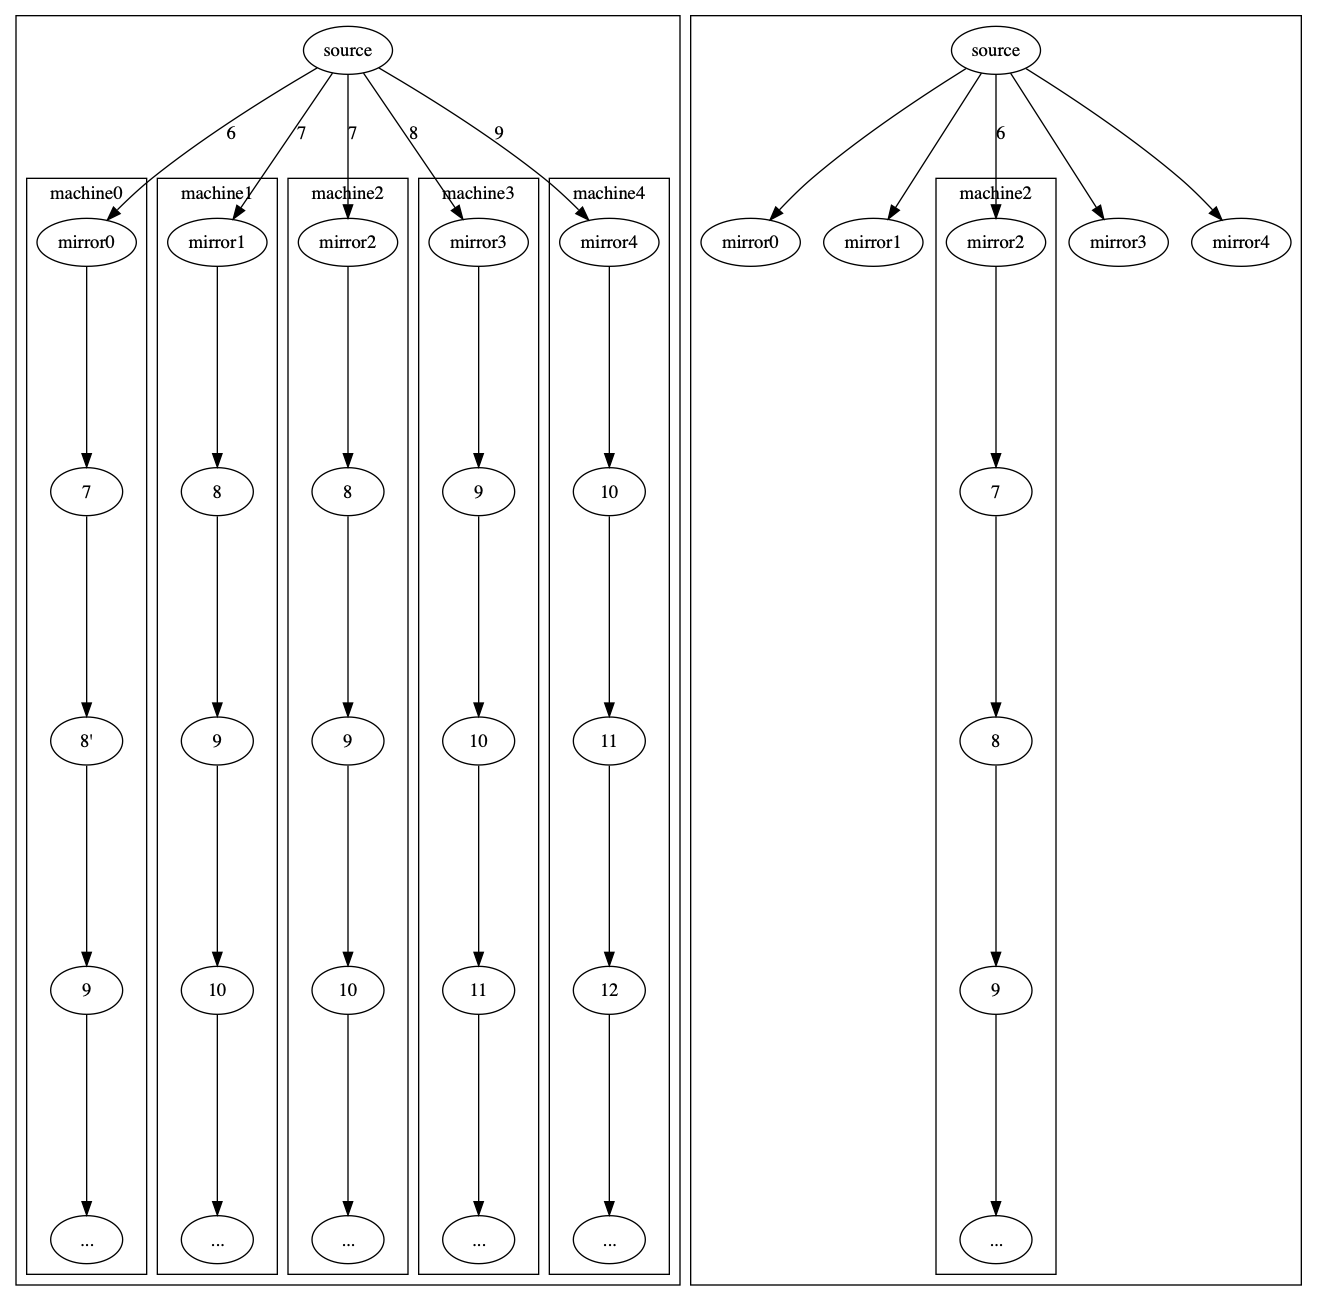
\includegraphics[width=0.5\textwidth]{Img/useless_and_local}
  \end{figure}
\end{frame}


\begin{frame}%解的局部性假设
  \frametitle{图计算过程中解的局部性规律}
  \begin{block}
    {图计算过程中的解的局部性规律:\\大多数活跃点的全局解都只由单个局部解构成}
    如下图所示,一些顶点有很多(10-28)个副本点,但全局解只由单个局部解构成。\\
    如果此时大部分顶点都是这样,那么此时开启延迟数据一致性方法就不会直接带来冗余计算。
  \end{block}
  \begin{figure}[H]
    \centering
    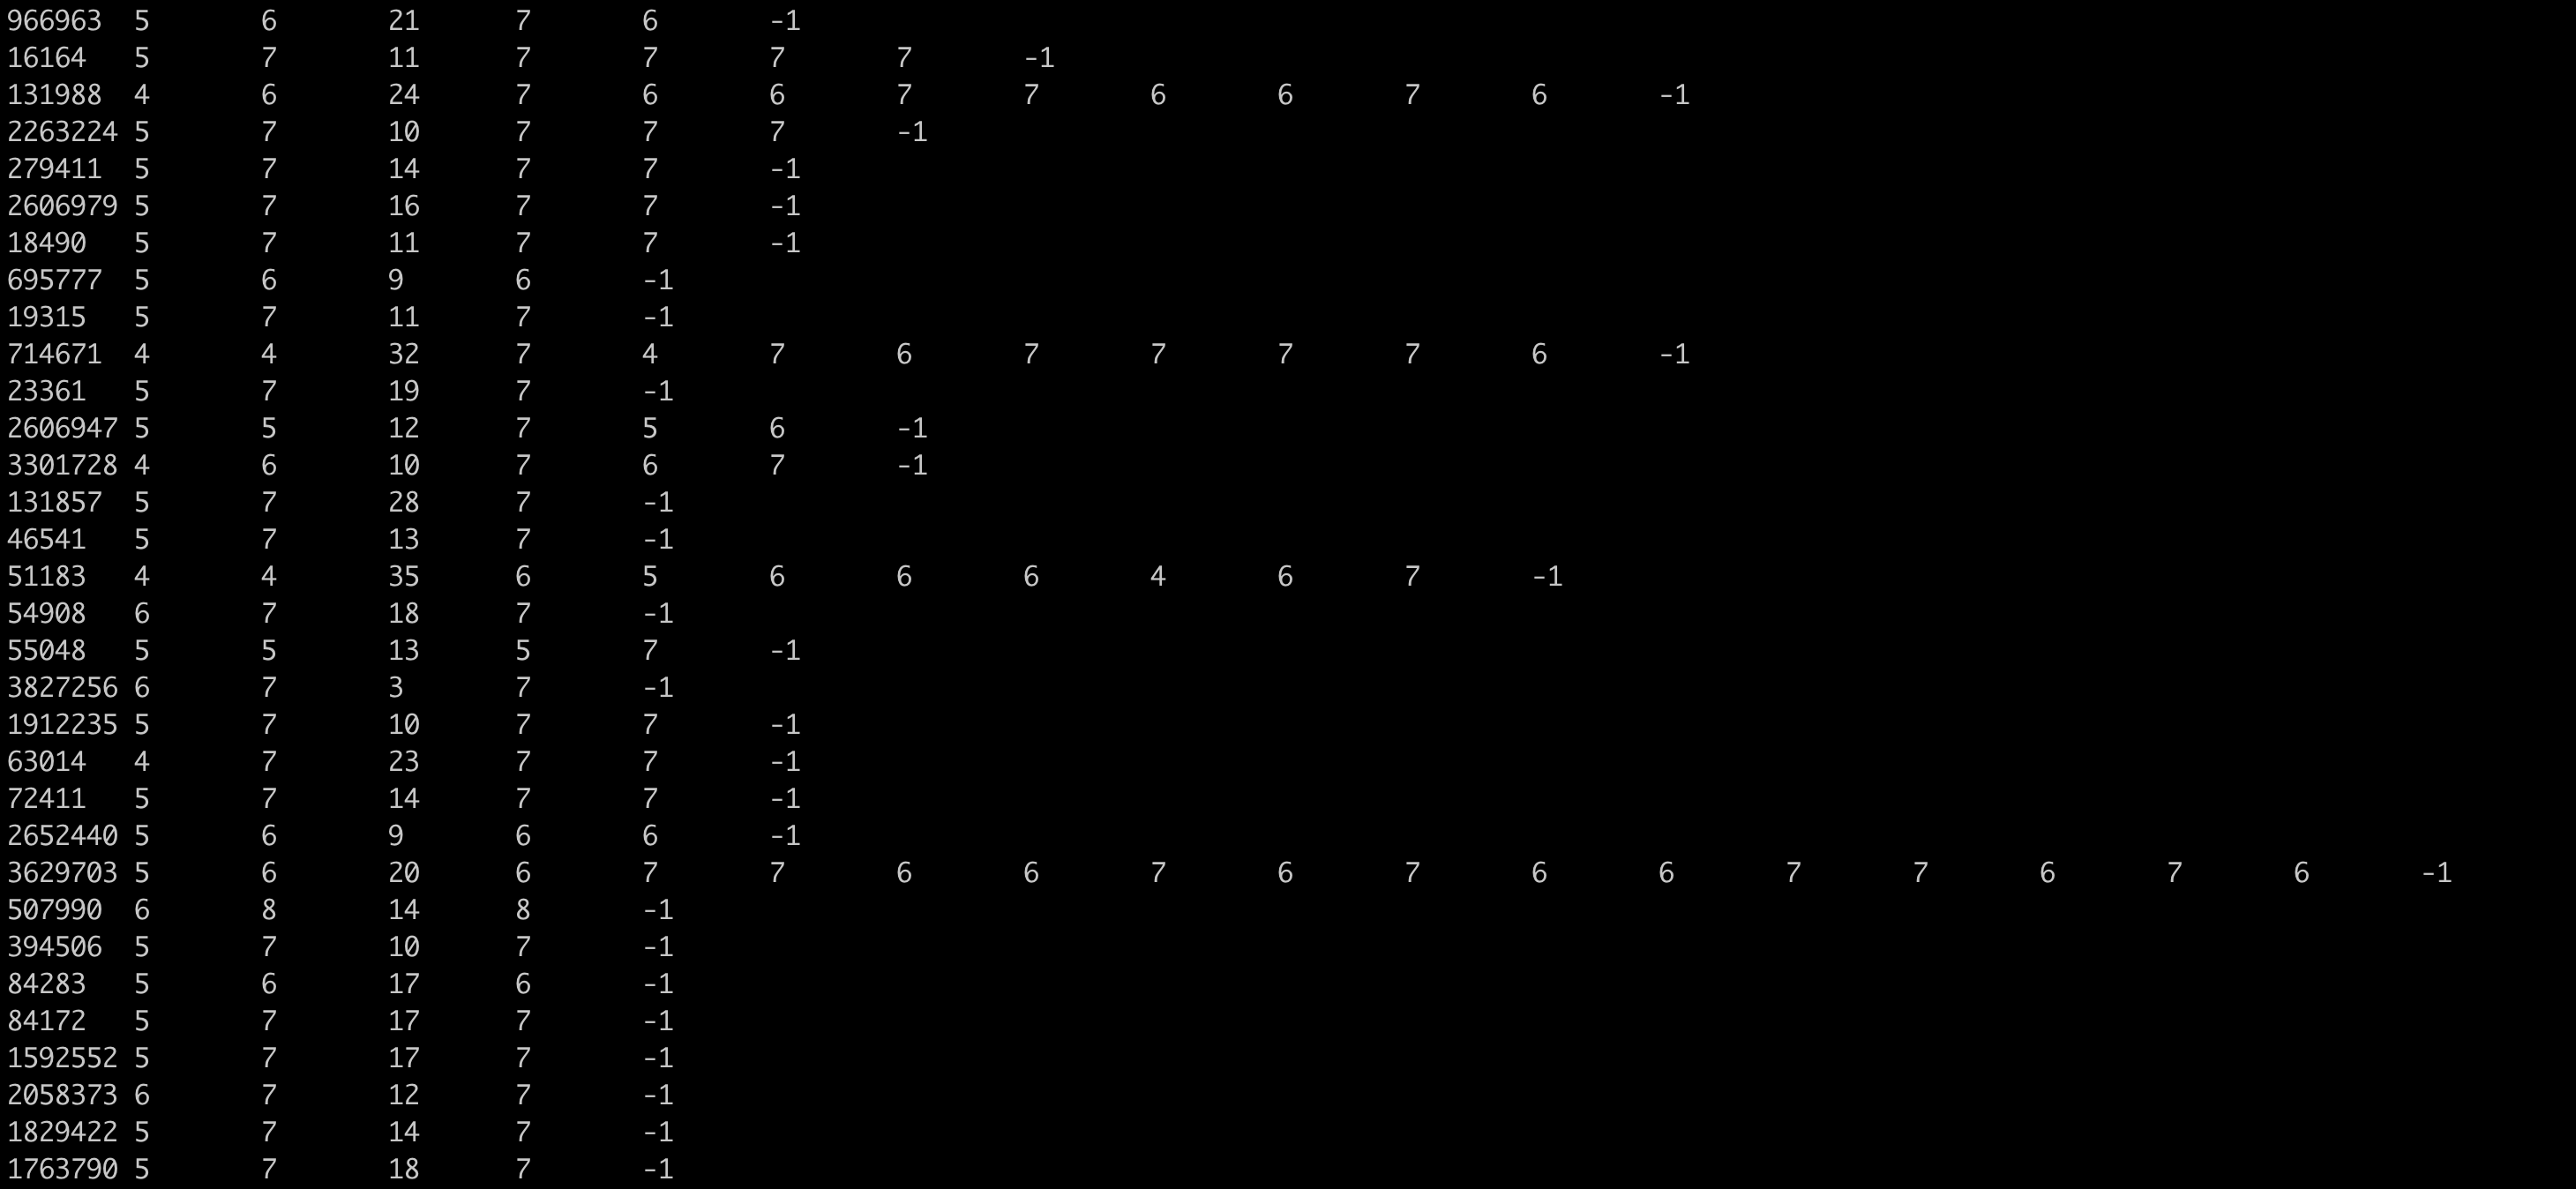
\includegraphics[width=0.8\textwidth]{Img/local_sssp}
    \caption[]{解的局部性示意图}
  \end{figure}
\end{frame}
\begin{frame}%如何观察全局解和局部解
  \frametitle{如何定量观察全局解和局部解}
  \begin{block}
    {}
    \begin{itemize}
      \item 局部解被包含在集群之间进行交换的消息累加和中
      \item 消息会被全部发送给标记为master的副本点
      \item 在顶点上添加两个数据结构可以记录第$i$次迭代的全局解和多个局部解
      \item 比较局部解和全局解之间的数值和数量关系可以统计判断\\
      每次迭代时解的局部性规律
    \end{itemize}
  \end{block}
  解决如何定量度量全局解和局部解之间的关系这一问题之后,本文在3种算法和8个输入图上进行了实验,得到如下结果。
\end{frame}


\begin{frame}%设计实验;实验结果
  \frametitle{实验结果-SSSP}

  \begin{figure}[H]
    \centering
    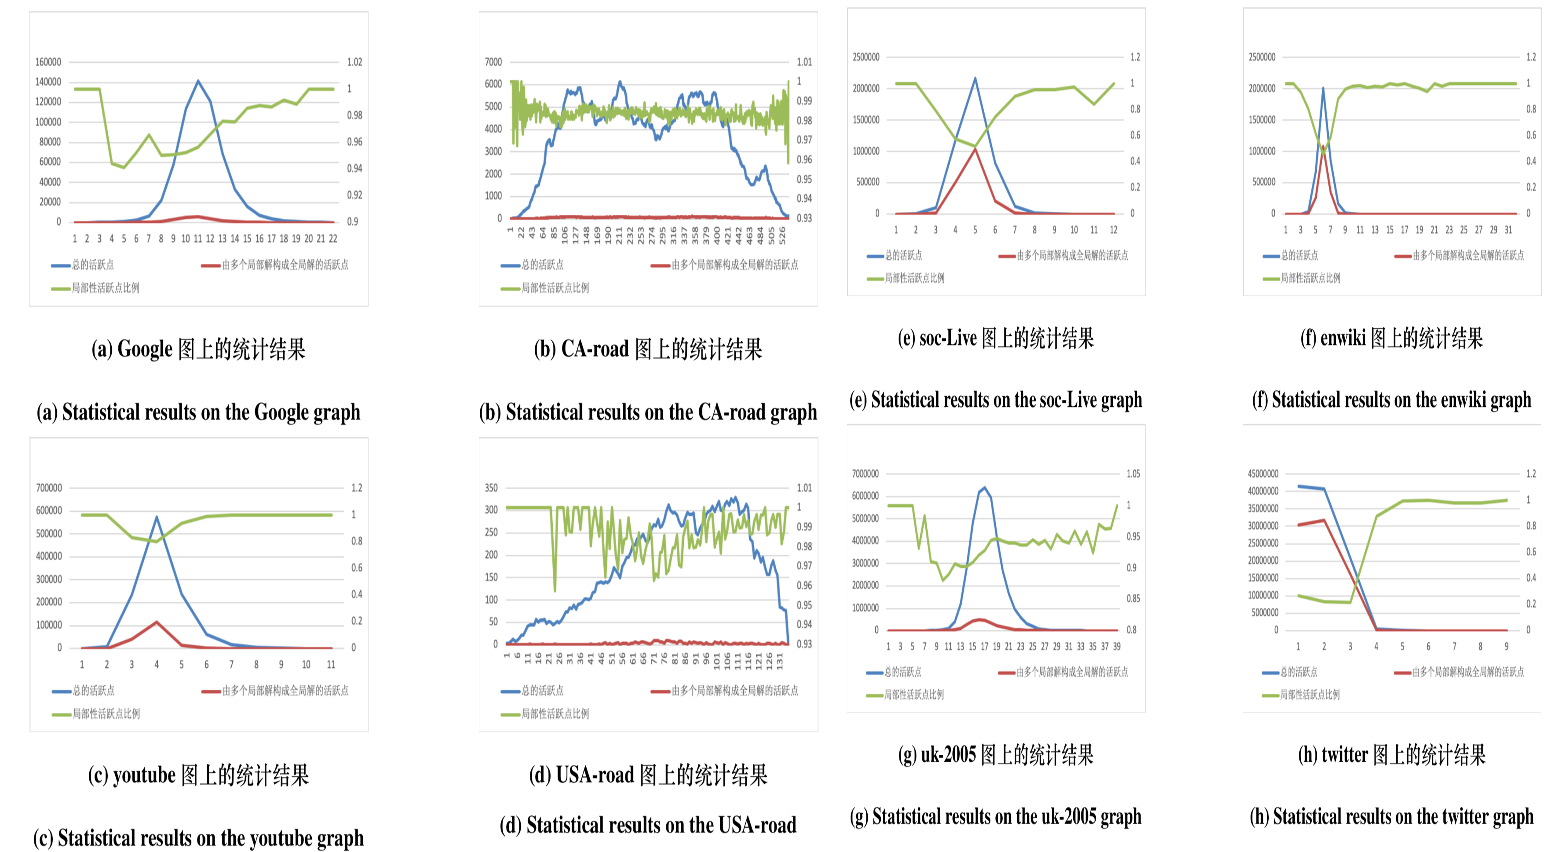
\includegraphics[width=0.9\textwidth]{Img/ppt_percent.png}
    \caption[]{SSSP 在8个输入图上解的局部性统计结果}
  \end{figure}
\end{frame}


\begin{frame}%设计实验;实验结果
  \frametitle{实验结果-CC}

  \begin{figure}[H]
    \centering
    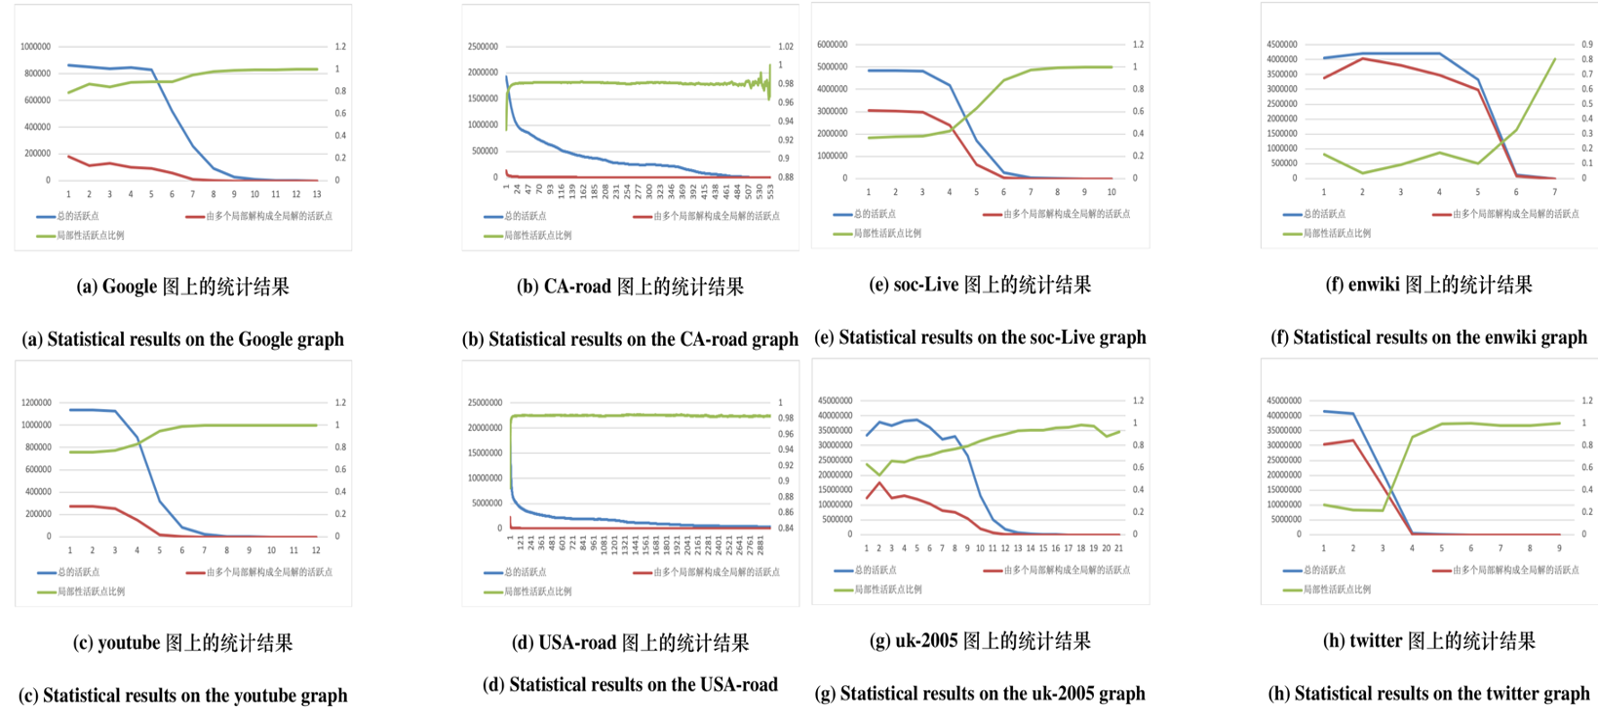
\includegraphics[width=0.9\textwidth]{Img/ppt_percent_cc.png}
    \caption[]{CC 在8个输入图上解的局部性统计结果}
  \end{figure}
\end{frame}


\begin{frame}%设计实验;实验结果
  \frametitle{实验结果-PageRank}

  \begin{figure}[H]
    \centering
    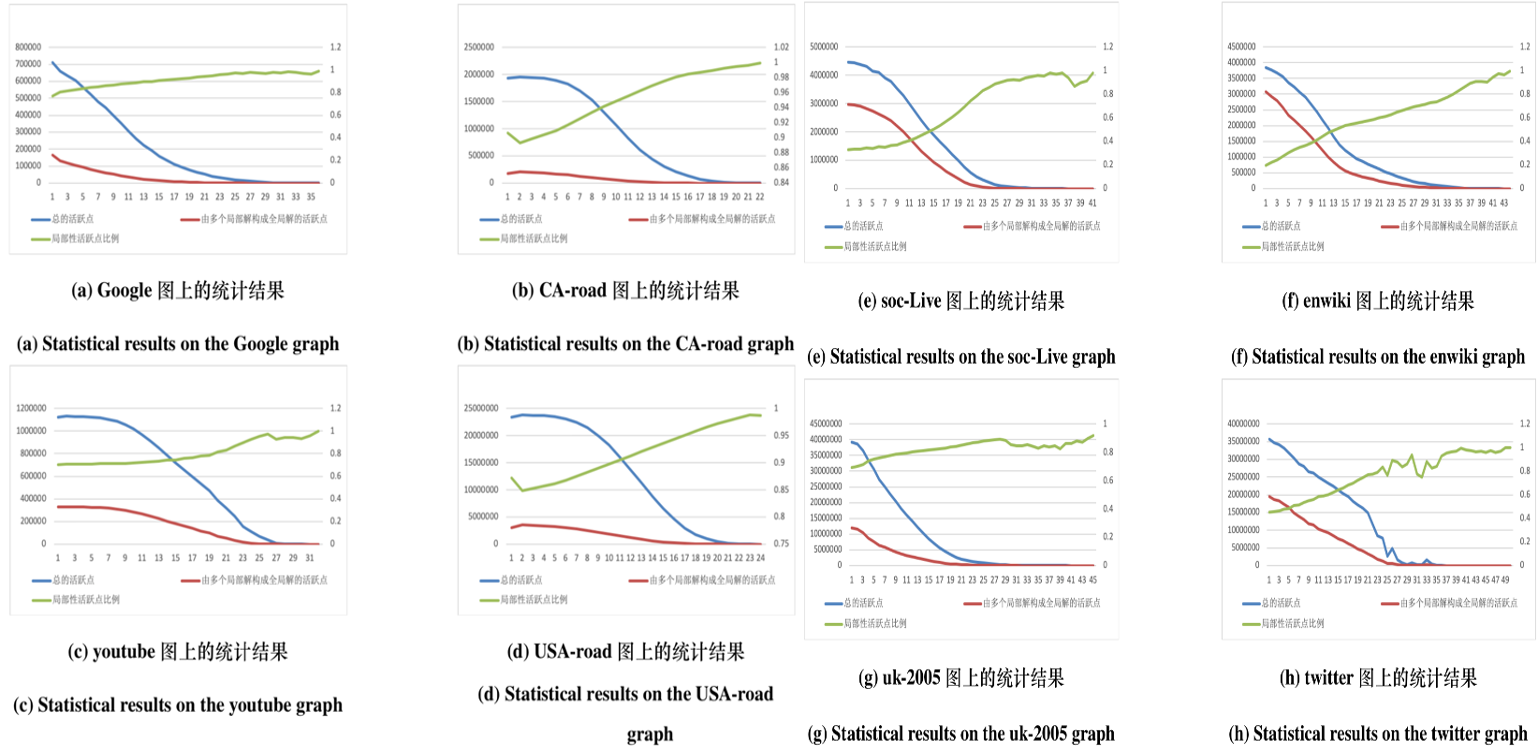
\includegraphics[width=0.9\textwidth]{Img/ppt_percent_pg.png}
    \caption[]{PageRank 在8个输入图上解的局部性统计结果}
  \end{figure}
\end{frame}

\begin{frame}%实验结果分析
  \frametitle{分析与结论}
  \begin{block}
    {实验数据分析}
    \begin{itemize}
      \item 在3种算法和8个输入图的24种组合中都存在着解的局部性规律:\\
      在每轮迭代的活跃点中大部分顶点的全局解都只由某个局部解构成,由多个构成的占极少数甚至没有。
      \item 在局部性较好($\frac{e}{v} \textless 10$)的图上,一开始就一直存在着明显的解的局部性:\\
      由单个局部解构成全局解的顶点的数量的比例维持在80\%-90\%以上
      \item 在局部性不好的图上,由单个局部解构成全局解的顶点的数量的比例在早期并不明显,到了后期才明显
      \item 局部性不好的图上,解的局部性规律开始出现的时刻和决策树的判断条件相一致
    \end{itemize}
  \end{block}
\end{frame}



\begin{frame}%实验结果分析
  \frametitle{分析与结论}
  \begin{block}
    {结论}
    图计算过程中普遍存在着解的局部性规律,但是这种规律的出现是动态的。\\
    在局部性好的图上,这种规律一开始就存在;在局部性不好的图上,这种规律在迭代一段时间后才出现。
  \end{block}
\end{frame}


\subsection{3:基于解的局部性的自适应优化方法}

\begin{frame}%如何在线统计解的局部性
  \frametitle{如何在线统计全局解和局部解的关系}
  \begin{block}
    {}
    通过研究结果2中的结论,我们知道,对于局部性好的图,我们可以选择直接开启的策略。
    对于局部性不好的图,我们则需要在线动态地识别出解的局部性规律的出现。

    \vspace{1em}

    考虑到解的局部性只是全局解和局部解之间的数量关系,我们不再需要观察具体的全局解和局部解。
    因此我们可以在消息交换过程中立即完成单个顶点上全局解是否由单个局部解构成的判断,然后通过
    $mpi.reduce$调用就能完成对一轮迭代中解的局部性的统计。
  \end{block}
\end{frame}


\begin{frame}%自适应优化方法-part 1
  \frametitle{基于解的局部性的自适应优化方法-part1}

  \begin{figure}[H]
    \centering
    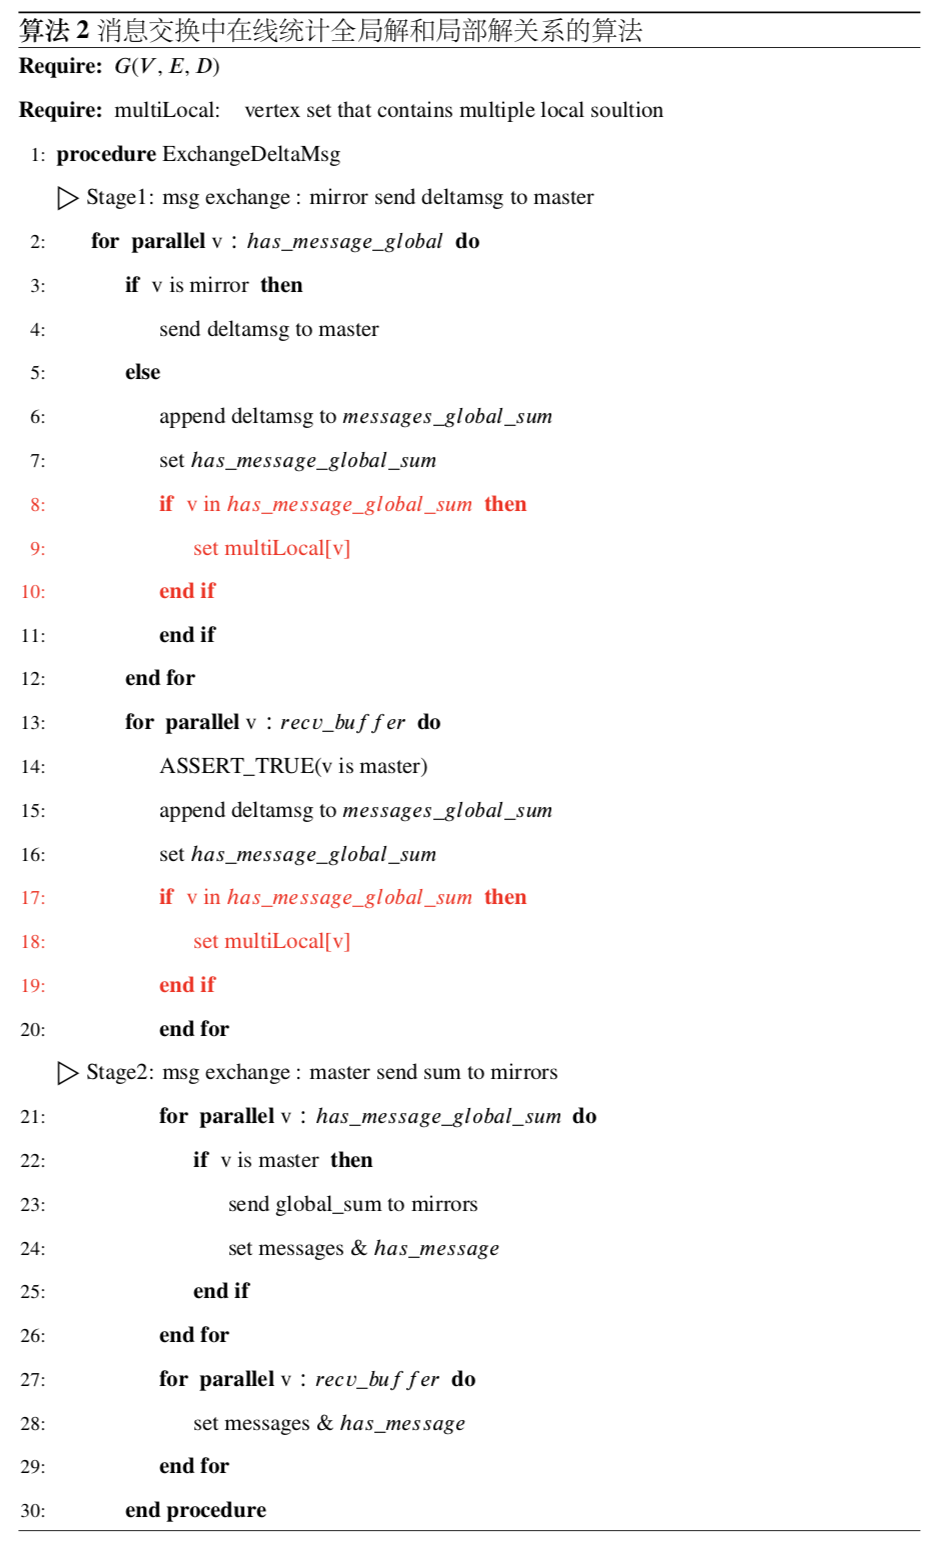
\includegraphics[width=0.48\textwidth]{Img/algo2.png}
  \end{figure}
\end{frame}


\begin{frame}%自适应优化方法-part 2
  \frametitle{基于解的局部性的自适应优化方法-part2}
  \begin{figure}[H]
    \centering
    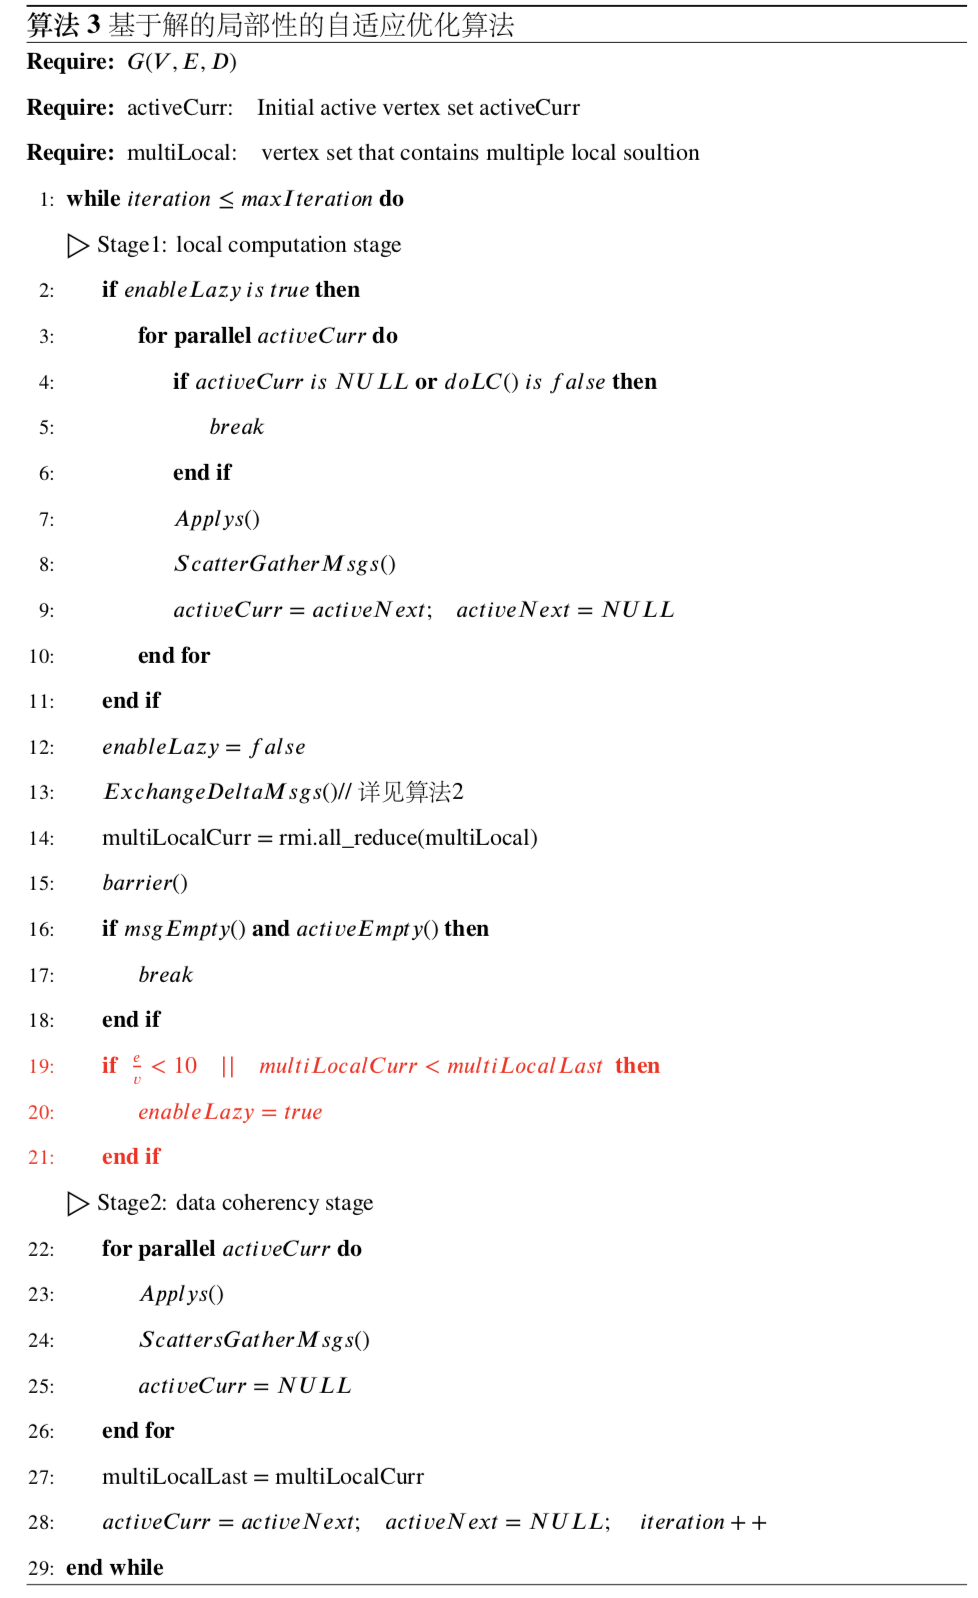
\includegraphics[width=0.48\textwidth]{Img/algo3.png}
  \end{figure}
\end{frame}



\begin{frame}%实验验证-结果;结果分析1
  \frametitle{实验结果}
  \vspace{-0.5em}
  \begin{figure}[H]
    \centering
    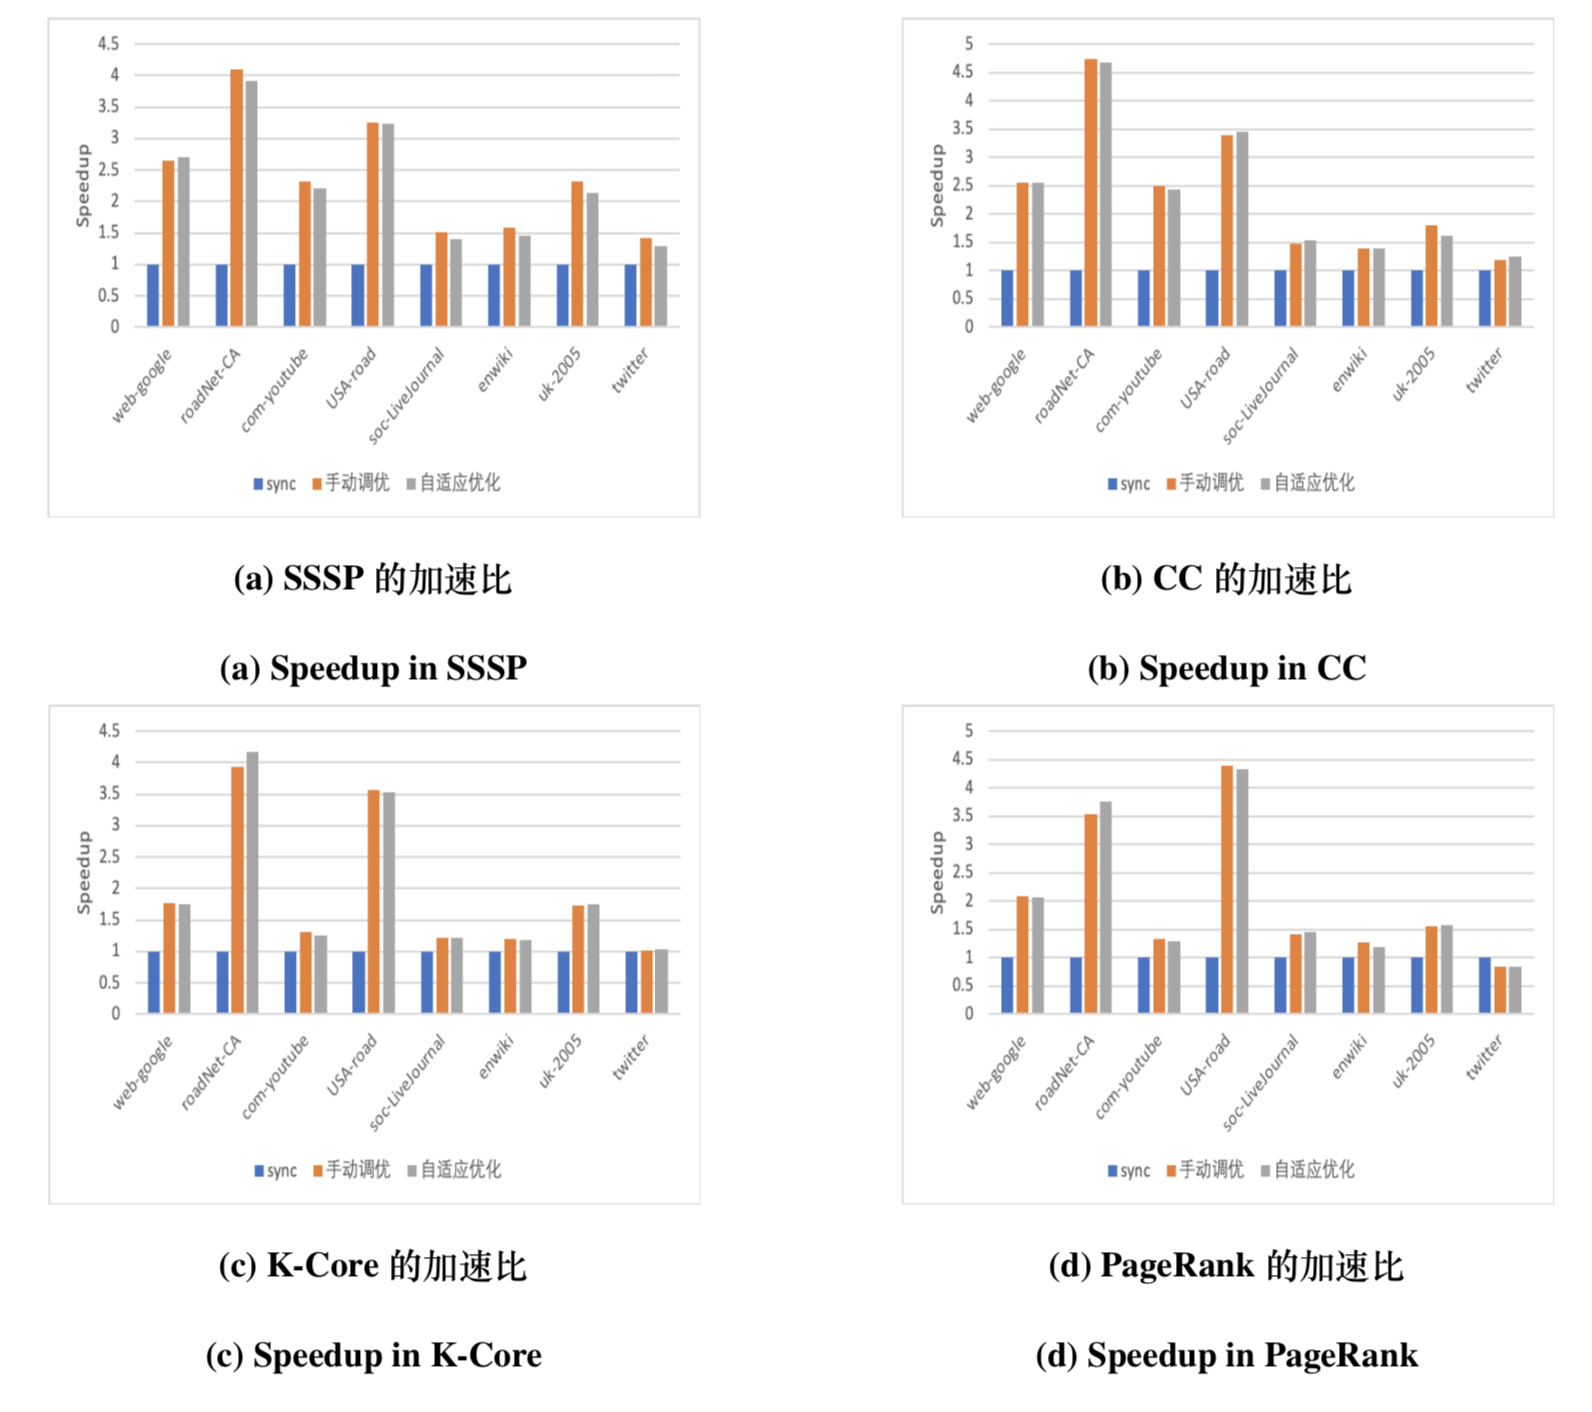
\includegraphics[width=0.8\textwidth]{Img/ppt_speedup.png}
    \caption[]{基于解的局部性的自适应优化算法在4种算法x8个输入图上的性能评测}
  \end{figure}
\end{frame}



\begin{frame}%实验验证-结果;结果分析1
  \frametitle{结果分析}
  \begin{center}
    基于解的局部性的自适应优化方法\\
    自动地得到了和手动调优相一致的性能提升效果
  \end{center}
\end{frame}

\section{总结与展望}

\begin{frame}%三个创新点
  \frametitle{总结}
  \begin{block}
    {本文的主要贡献可以总结为以下三个方面}
    \begin{enumerate}
      \item  对LazyAsync的在不同开启策略下得到不同性能提升这一现象进行了研究,认清了这一方法的性能提升规律。
      \item 对图计算过程中活跃点上全局解和局部解之间的关系进行了研究,发现了解的局部性这一现象。
      \item 基于解的局部性这一现象,实现了基于解的局部性的自适应优化方法。
      这种方法解决了LazyAsync在不同的输入条件下如何得到相对最优的性能提升这一问题。
    \end{enumerate}
  \end{block}
\end{frame}


\begin{frame}%后续工作
  \frametitle{展望}
  本文是对LazyAsync的延续和补充。\\
  本文的工作解决了这种方法的自适应优化问题,使得 LazyAsync 真正成为了一个完善而实用的方法。

  在后续的研究中,可以考虑把这种方法移植到其他分布式图计算系统中去。
\end{frame}



\begin{frame}%end
  \begin{center}
    \begin{huge}
      谢谢\\[\baselineskip]
      请各位老师批评指正          
    \end{huge}
  \end{center}
\end{frame}
\end{document}